\documentclass{beamer}
\usepackage[utf8]{inputenc}
\usepackage[T1]{fontenc}
\usepackage{graphicx}
\usepackage{color}
\usepackage{hyperref}
\usepackage[all]{xy}
\usepackage{tikz}
\usepackage{wasysym}

\usetikzlibrary{shapes.callouts}
  
\setbeamertemplate{frametitle continuation}[from second]

% \mode<presentation>
% {
%   \usetheme{Warsaw}
%   % or ...

%   \setbeamercovered{transparent}
%   % or whatever (possibly just delete it)
% }


\title{Why property-based testing matters}

\author[Pedro Vasconcelos]{Pedro Vasconcelos \\ \texttt{pbvascon@fc.up.pt}}

\institute[LIACC, DCC/FCUP]{
  DCC/FCUP \& LIACC \\
  
\includegraphics[width=0.4\textwidth]{images/fcup-identidade-logotipo-cores}
  \qquad
  \raisebox{4ex}{
\includegraphics[width=0.3\textwidth]{images/liacc-logo.png}}
}

\date{6th December 2024}

\newcommand{\bs}{\symbol{92}}

% discard trial for counter-example
\newcommand{\counter}[1]{\textbf{#1}}
\newcommand{\noncounter}[1]{{\mathtt{#1}}}


% If you have a file called "university-logo-filename.xxx", where xxx
% is a graphic format that can be processed by latex or pdflatex,
% resp., then you can add a logo as follows:

% \pgfdeclareimage[height=0.5cm]{university-logo}{university-logo-filename}
% \logo{\pgfuseimage{university-logo}}



\begin{document}

\begin{frame}
  \titlepage
\end{frame}


\begin{frame}
  \frametitle{Overview}
  
  \begin{itemize}
  \item A long-standing challenge for software engineering 
    is ensuring software correctness
  \item Formal verification is (still) expensive and rarely used
  \item \emph{Tests} are the most commonly used
    practical technique 
  \item \emph{Unit tests} are the industry-standard
    for verification ``in the small''
  \end{itemize}
\end{frame}

\begin{frame}{This talk}
  
  \begin{itemize}
  \item \emph{Property-based testing}: an
    automatic testing alternative to unit tests
  \item A ``lightweight'' formal method
  \item Available for many programming languages
  \item Many successful applications in open-source and some industrial
    projects
  \item But still not commonly taught and under-utilized in practice
  \end{itemize}
\bigskip
   Slides and demo code: \url{https://github.com/pbv/why-pbt-matters}
\end{frame}

\begin{frame}
  \frametitle{``Lightweight'' formal method?}
\framesubtitle{According to Benjamin Pierce, author of \emph{Types and Programming Languages}}
  \bigskip\bigskip
  \begin{block}{Formal method\tikz[remember picture]\node(a){\vphantom{X}};}
    ``A mathematically rigorous technique for validating the actual
    behaviour of a program against a description of desired behavious.''
\end{block}
  \bigskip\bigskip

  \begin{block}{Lightweight formal method\tikz[remember picture]\node(b){\vphantom{X}};}
    ``One that can be applied successfully by someone who doesn't fully
    understand it.'' \smiley
  \end{block}
  
  \begin{tikzpicture}[remember picture,overlay]
    \path<2> (a.east) ++(0,1) node[anchor=west,ellipse callout,fill=red!50,opacity=.5, callout absolute pointer={(a.mid)}]{supports automation};
    \path<2> (b.east) ++(0,1) node[anchor=west,ellipse callout,fill=red!50,opacity=.5, callout absolute pointer={(b.mid)}]{requires automation};   
  \end{tikzpicture}
\end{frame}

\begin{frame}[fragile]
  \frametitle{PBT vs unit tests vs formal verification}
  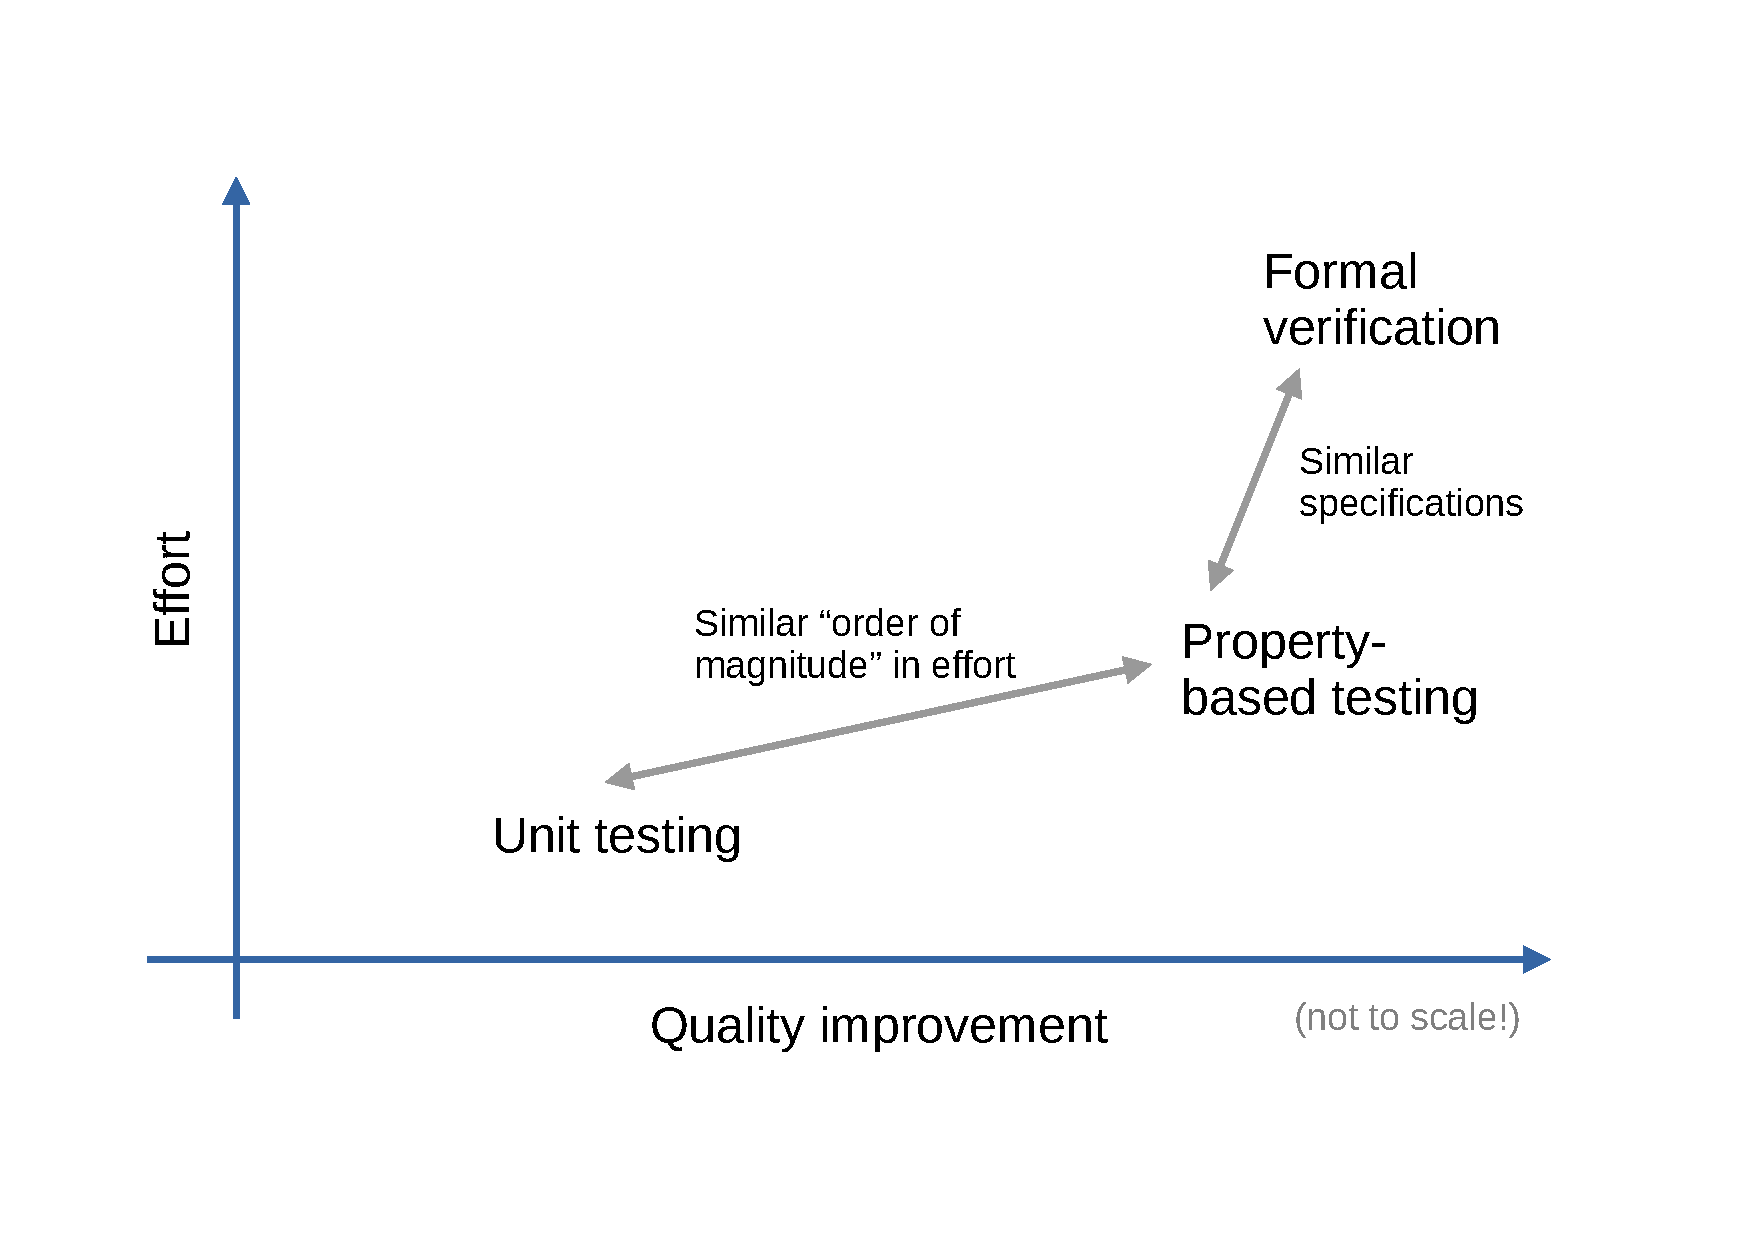
\includegraphics[width=\textwidth]{images/pbt-vs-formal} 
\end{frame}



\begin{frame}[fragile]
  \frametitle{Unit tests}
\begin{itemize}
\item Code fragments for testing functions, classes, libraries, etc.
\item Express the expected outputs for specific combinations of inputs
\item Example: testing an integer square root function in Python
\begin{verbatim}
def test_isqrt():
   assert isqrt(0) == 0
   assert isqrt(2) == 1
   assert isqrt(4) == 2
   assert isqrt(5) == 2
   assert isqrt(9) == 3
\end{verbatim}
\end{itemize}
\end{frame}


\begin{frame}[fragile]
  \frametitle{Problems with unit tests}

  Cognitive bias:
  \begin{itemize}
  \item how can we include an edge case in the tests
    that we didn't consider in the code?
  \end{itemize}
  \medskip
  
  Poor scaling:
  \begin{itemize}
  \item a few unit tests per feature
  \item for $n$ features, $O(n)$ unit tests
  \item but testing \emph{interactions} between features requires $O(n^2),
    O(n^3), \ldots$ unit tests
  \end{itemize}
  \pause
  \bigskip
  

    \begin{minipage}{0.7\textwidth}
      Solution:
      \medskip
      
      \begin{quote}
        ``Don't write tests 
        --- generate them!''
      \end{quote}
      John Hughes, co-author of the \emph{QuickCheck}
      PBT library
    \end{minipage}
    \begin{minipage}{0.25\textwidth}
      \hfill
      
\includegraphics[width=0.8\textwidth]{images/john-hughes}
    \end{minipage}  
\end{frame}


\begin{frame}[allowframebreaks]
  \frametitle{Property-based testing}

\begin{itemize}
\item Write \emph{properties} instead of specific tests
\begin{itemize}
\item should be universal, i.e.\@ hold for all values
\item should define the expected behaviour for \emph{all} cases
\end{itemize}
\item Specify \emph{generators} for the inputs
\item The testings framework runs the property with
  a large number of inputs
  \begin{itemize}
  \item testing fails if a \alert{counter-example} is found
  \item otherwise, testing succeeds
  \end{itemize}
\end{itemize}

\framebreak

\begin{itemize}
\item QuickCheck (2000): first PBT library (for Haskell)
\item Other implementations:
  \begin{description}
  \item[PropEr] for Erlang
  \item[ScalaCheck] for Scala
  % \item[Hedgehog, Falsify] for Haskell
  \item[Hypothesis] for Python
  \item[FsCheck] for F\#
  \item[JUnit-QuickCheck] for Java
  \item[RapidCheck] for C++
  \end{description}
\end{itemize}
\bigskip

Many others: \url{https://en.wikipedia.org/wiki/QuickCheck}
\end{frame}

\begin{frame}[fragile]
  \frametitle{Example property}

  What can we say about the integer square root function?
  \pause
  \medskip

  Let $n$ be an arbitrary non-negative number;
  let $r = \texttt{isqrt}(n)$; then
  \[ r\geq0 \land r^2 \leq n \land (r+1)^2>n  \]
  i.e.\@ $r$ should be \emph{largest non-negative integer} such that
  $r^2 \leq n$.
  \pause
  \medskip

  In Python:
\begin{semiverbatim}
from hypothesis import given
import hypothesis.strategies as st
@given(\alert<5>{st.integers(min_value=0)})  \only<5->{\textsl{# non-negative integer}}
def test_isqrt(\alert<4>{n}):                \only<4->{\textsl{# for all n}}
    r = isqrt(n)
    assert \alert<6>{r>=0 and r**2<=n and (r+1)**2>n}   \only<6->{\textsl{# assertion}}
  \end{semiverbatim}

  \visible<7>{\hfill (Cue demo.)}
  
\end{frame}

\begin{frame}
  \frametitle{Properties in Hypothesis}

  \begin{itemize}
  \item Properties are \emph{functions}\ldots
  \item \ldots that should fail if the expected condition is not met
  \item Arguments are \emph{universally quantified}
  \item For each property:
    \begin{itemize}
  \item test with a large number of random values (100 by default)
  \item generated using \emph{strategies}
  (defined by \texttt{@given})
    \end{itemize}
  \item Module \texttt{hypothesis.strategies} provides:
    \begin{itemize}
    \item \emph{predefined strategies} for basic types
    \item methods for \emph{modifying} and \emph{combining} strategies
    \end{itemize}
  \end{itemize}
\end{frame}



\begin{frame}
  \frametitle{Strategies}

  \begin{description}
    \item[floats()] generate floating-point numbers
  \item[integers()] generate integers
  \item[booleans()] generate logical values 
  \item[text()] generate Unicode strings
  \item[lists($s$)] lists of elements given by strategy $s$
    % \item[tuples($s1,s2,\ldots$)] lists of elements given by strategies $s1,s2,\ldots$
    \item[\ldots] many others
  \end{description}
  \bigskip
  
  We can also:
  \begin{itemize}
  \item customize strategies using \emph{parameters} (e.g.\@ \texttt{min\_value})
  \item modify strategies by \emph{mapping} and \emph{filtering}
  \item combine stategies using \emph{combinators}
  % \item sample them using the \texttt{.example()} method    
  \end{itemize} 
\end{frame}


\begin{frame}[fragile]
  \frametitle{Generating data}

\begin{verbatim}
>>> integers().example()
848041

>>> lists(integers(min_value=0, max_value=100)).example()
[2, 29, 54, 66, 1, 27, 77, 81, 51, 18, 18]

>>> lists(integers().map(lambda x:x*2)).example()
[6668, -38, 1081651134, -6590]

>>> lists(integers()).map(sorted).example()
[-6913, -59, 37, 77, 90, 25088]

>>> lists(one_of(integers(), booleans())).example()
[True, True, -1318, True, True, -46, -46, True, -46]
\end{verbatim}
\end{frame}


\begin{frame}
  \frametitle{Another example}

  Let's test the interaction between \emph{list reverse}
  and \emph{append}.
  
  Consider $x, y$ two arbitrary lists:

  \[  reverse(x + y) = \alt<1>{\hspace{2ex}???\hspace{18ex}}{reverse(y) + reverse(x)} \]
  \pause

  Example:
  \[\begin{array}{ll}
      reverse([1,2] + [3,4]) &= reverse([3,4]) + reverse([1,2]) \\
                             &= [4,3] + [2,1]\\
                             &= [4,3,2,1]
  \end{array}\] 
\end{frame}

\begin{frame}[fragile]
  \frametitle{Testing with lists of integers}

\begin{verbatim}
intlist = st.lists(st.integers())
@given(intlist, intlist)
def test_reverse_append(x, y):
    assert reverse(x + y) == reverse(x) + reverse(y)
\end{verbatim}
\medskip
\pause
  
\begin{semiverbatim}
pytest basic.py -k test_reverse_append

==================== FAILURES ==========================
\alert{______________ test_reverse_append _____________________}

x = [0], y = [1]
\end{semiverbatim}
What happened\ldots ?  
\end{frame}

\begin{frame}[fragile]
  \frametitle{Checking expectations}


\begin{itemize}
\item We've written the property incorrectly!
\begin{semiverbatim}
  assert reverse(x + y) == reverse(\alert{x}) + reverse(\alert{y})
      \textsf{instead of}
  assert reverse(x + y) == reverse(y) + reverse(x)  
\end{semiverbatim}
\item Hypothesis found a counter-example for the wrong property:
   \[ reverse([0]+[1]) \neq reverse([0]) + reverse([1]) \]
\item This is the \emph{smallest} counter-example
  that falsifies the property
\item Hypothesis \emph{always} find this counter-example
  regardless of random generation!
\end{itemize}
\end{frame}


\begin{frame}
  \frametitle{Shrinking}

  \begin{itemize}
  \item Hypothesis attempts to simplify counter-examples
  before presenting; e.g.:
  \begin{itemize}
  \item removing elements from the lists
  \item shrinking elements inside the lists
  \end{itemize}
\item This is useful to remove ``noise'' from
  randomly generated data
\item For the previous example we obtain
  the \emph{minimal} counter-example  
\item In general, shrinking only finds a \emph{local minimum}
\end{itemize}
\end{frame}


\begin{frame}[fragile,allowframebreaks]
  \frametitle{A real-world example}
  \begin{itemize}
  \item Erlang code for SMS text packing at Ericsson
  \item 7-bit characters transmitted using 8-bit \emph{bytes}
  \item GSM standard: pack 8 caracteres into 7 bytes
\item Two functions (translated to Python):
\begin{verbatim}
pack(seq: bytes) -> bytes
unpack(seq: bytes) -> bytes
\end{verbatim}
\item Roundtrip property: unpack is the inverse of pack
  \[ unpack(pack(seq)) = seq, ~\text{for all}~ seq \]
\end{itemize}

\framebreak

  \begin{itemize}
  \item John Hughes's company (QuviQ) found a subtle bug 
    affecting strings of length multiple of 8
    ending in a \texttt{\bs NUL} character
  \item The code had been unit tested and  was in production
  \end{itemize}
\end{frame}


\begin{frame}[allowframebreaks]
  \frametitle{Validating AI generated code}

    \begin{center}
\includegraphics[width=0.75\textwidth]{images/rle_chat.png}
  \end{center}
  
  \begin{itemize}
  \item Let us use Hypothesis to validate AI generated code
  \item Problem: write a pair of encode/decode functions
    for \alert{run-length encoding}   
  \end{itemize}

  \[ \xymatrix@-0.5pc {
      \texttt{'AAABBCAAAAA'}\ar@/^/[rr]^{encode} &
      & \texttt{'A3B2C1A5'}\ar@/^/[ll]^{decode}
    }
  \]

\end{frame}

\begin{frame}[fragile]
  \frametitle{Testing ChatGPT solution}

  \begin{block}{``Roundtrip'' property i.e.\@ decode is the inverse of encode}
\begin{verbatim}
@given(st.text())
def test_decode_encode_1(s):
    assert rle_decode(rle_encode(s)) == s
\end{verbatim}
    \end{block}\pause


\begin{semiverbatim}
pytest rle_tests.py -k test_decode_encode_1
=================== FAILURES ===========================
\alert{_____________ test_decode_encode_1 _____________________}

s = '01'
\end{semiverbatim}

The solution doesn't work for strings with digits!
  
\end{frame}

\begin{frame}[fragile]
  \frametitle{Characterizing failure}

  We can check if the generated code
  works when the string contains no digits:
\begin{verbatim}
no_digits = st.characters(exclude_categories='N')
@given(st.text(alphabet=no_digits))
def test_decode_encode_2(s):
    assert rle_decode(rle_encode(s)) == s
\end{verbatim}

  \begin{itemize}
  \item The property now passes the default 100 tests
  \item We could now try to fix the solution for digits
  \item But first: perform some statistics on the testing data
  %   \begin{itemize}
  %   \item try to fix the solution for digits 
  %   \item perform statistics on test data
  %   \item improve test data distribution
  %   \end{itemize}
  % \item This greatly increases the trust in the generated code
  \end{itemize}
\end{frame}

\begin{frame}[fragile,allowframebreaks]
  \frametitle{Characterizing test data}

\begin{verbatim}
def longest_count(s: str) -> int:
   "Compute the maximum length of repeated chars."
   ...

@given(st.text(alphabet=no_digits))
def test_decode_encode_3(s):
    event(f'longest = {longest_count(s)}')
    assert rle_decode(rle_encode(s)) == s
\end{verbatim}

  \framebreak
  
\begin{semiverbatim}
pytest rle_tests.py -k test_decode_encode_3 \\
        -{}-hypothesis-show-statistics

================== Hypothesis Statistics ===============
      * 75.70%, longest = 1
      * 22.69%, longest = 2
      * 1.00%, longest = 0
      * 0.60%, longest = 3
\end{semiverbatim}

\begin{itemize}
\item 75\% of the test cases had no repeats
\item 22\% had maximum of 2 repeats
\item No test case had more than 3 repeats
\item Why? Because \texttt{text()} 
   chooses each character independently
\end{itemize}
\end{frame}

\begin{frame}[fragile,allowframebreaks]
  \frametitle{Improving test data generation}

  We will use \alert{combinators} to write a strategy that:
  \begin{enumerate}
\item generates a long sequence of a \emph{single repeated} character;
\item \emph{or} generates text as before.
\end{enumerate}
\bigskip

\begin{verbatim}
many_no_digits
  = st.builds(lambda count, char: count*char,
              st.integers(min_value=0, max_value=20),
              no_digits)

combined = st.one_of(many_no_digits,
                     st.text(alphabet=no_digits))
\end{verbatim}

\framebreak

This gives much better test data distribution:

\begin{center}
\begin{minipage}{0.5\textwidth}
{\small\begin{verbatim}
      * 35.69%, longest = 1
      * 12.90%, longest = 2
      * 10.48%, longest = 3
      * 5.44%, longest = 0
      * 4.23%, longest = 20
      * 4.23%, longest = 6
      * 3.63%, longest = 4
      * 3.23%, longest = 7
      * 3.02%, longest = 8
      * 2.82%, longest = 12
\end{verbatim}}
\end{minipage}\begin{minipage}{0.45\textwidth}
{\small\begin{verbatim}
      * 2.82%, longest = 14
      * 2.82%, longest = 17
      * 1.81%, longest = 9
      * 1.61%, longest = 10
      * 1.61%, longest = 13
      * 1.41%, longest = 15
      * 1.21%, longest = 19
      * 0.60%, longest = 5
      * 0.40%, longest = 18
\end{verbatim}}
\end{minipage}
\end{center}

\end{frame}

\begin{frame}[allowframebreaks]
  \frametitle{Conclusion}

\begin{itemize}
\item PBT philosophy: write \emph{properties} and \emph{generate} tests
\item Lightweight: implemented as libraries
\item Flexible: domain-specific languages (DSLs) for writing
    data generators and properties
 \item Scales to realistic software   
\item Couples executable specifications with code
\item Useful for comunicating expectations among developers
\item Useful for finding subtle bugs in complex systems 
\end{itemize}
\end{frame}



\begin{frame}
  \frametitle{Challenges}
\begin{itemize}
\item Writting \emph{effective} properties  
  \begin{itemize}
  \item training software engineers to think about
    pre- and post-conditions, invariants, etc.
  \item universities can play a significant role here
  \item helping industry adopt a higher-skill technology 
  \end{itemize}
\item PBT works best with software that is well structured
\item Design systems around properties and not the other way around
% \item Is validation of AI~generated code a ``killer app''
%  for PBT? 
\end{itemize}
\end{frame}

\begin{frame}
  \frametitle{References}

  \begin{thebibliography}{9}
  \bibitem{quickheck} K. Claessen and J. Hughes.
    \emph{QuickCheck: A lightweight tool for random testing of Haskell
      programs}, ACM ICFP 2000
  \bibitem{hypothesis} D. R. MacIver \emph{et al}.
    \emph{Hypothesis: A new approach to property-based testing},
    The Journal of Open Source Software, 2019.
    See also \url{https://hypothesis.readthedocs.io/}
  \bibitem{telecoms} T. Arts, J. Hughes and J. Johansson
    \emph{Testing Telecoms Software with Quviq QuickCheck},
    ACM Workshop on Erlang, 2006
  \bibitem{autosar} T. Arts, J. Hughes, U. Norell and H. Svensson,
    \emph{Testing AUTOSAR software with QuickCheck}, IEEE ICSTW 2015
  \bibitem{practice} H. Goldstein, \emph{et al}. \emph{Property-Based
      Testing in Practice}, IEEE/ACM ICSE 2024
  \end{thebibliography}


\end{frame}

\begin{frame}
\begin{center}
  \Huge Extra slides
\end{center} 
\end{frame}


\begin{frame}
  \frametitle{Writing properties}

  \begin{description}
  \item[equivalence] $f(x) = f_{spec} (x)$
  e.g.\@ $f(x)$ is an optimized implementation
  and $f_{spec}(x)$ is a reference implementation.
    
  \item[idempotency] $f(f(x)) = f(x)$
  \item[inverse]  $g(f(x)) = x$ 
  \item[associativity] $f(x,f(y,z) = f(x,y),z)$
  \item[commutativity] $f(x,y) = f(y,x)$
  \item[right identity] $f(x,zero) = x$
  \item[left identity] $f(zero,x)= x$
  \end{description}
  \bigskip

  Hypothesis can write these kind of properties for you ---
  see \texttt{hypothesis.ghostwriter}.

\end{frame}


\begin{frame}
  \frametitle{Stateful programs}

We can also use PBT to test programs that:
\begin{enumerate}
\item modify state;
\item read and write files;
\item use network services, databases, etc.
\end{enumerate}
\end{frame}

\begin{frame}
  \frametitle{Testing stateful programs}

\begin{itemize}
\item Generate sequences of commands
\item Specify behaviour using a functional model (state machine)
\item Compare the execution against the model
\end{itemize}

\begin{center}
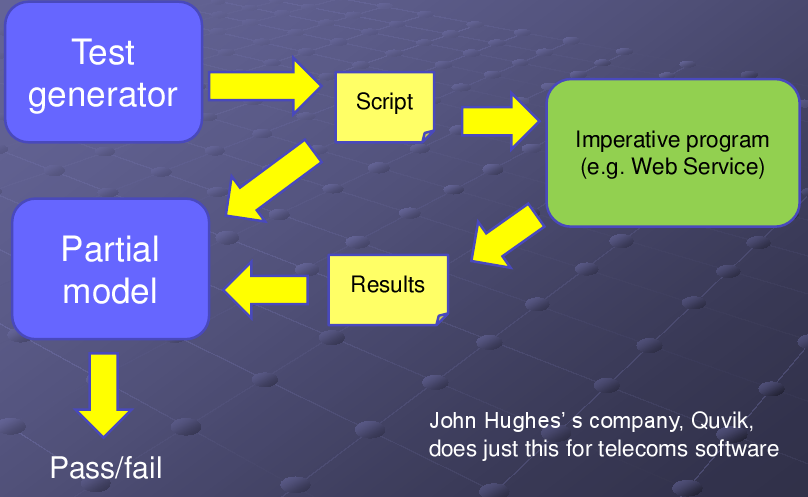
\includegraphics[width=0.75\textwidth]{images/imperative.png}
\end{center}
\end{frame}



\begin{frame}
  \frametitle{Industrial use example}

\begin{itemize}
\item Ericsson Media proxy (Java and C++)
\item Establish telephony connection throught a firewall
\item Tested with Erlang QuickCheck (Quviq.com)
\item Adding and removing participants in a call
\item Random counterexample with 160 commands
\item Shrunk automatically to 7 commands
\end{itemize}

\begin{center}
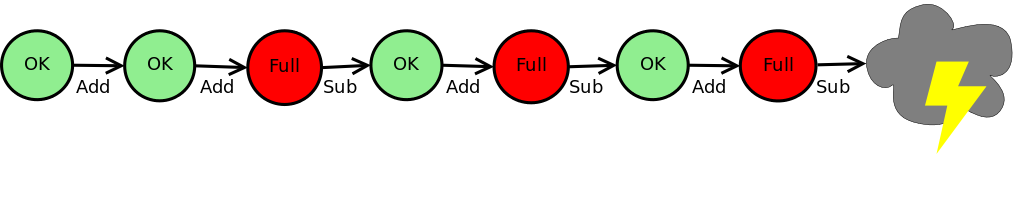
\includegraphics[width=\textwidth]{images/media1}
\end{center}
\end{frame}

\end{document}

